\documentclass[11pt]{extarticle}
\usepackage{unicode-math}
\usepackage{mathrsfs}
\usepackage{amsthm,graphicx,xcolor,natbib,enumitem,booktabs,tabularx}
\usepackage[paperwidth=126mm, paperheight=96mm, top=5mm, bottom=5mm, right=5mm, left=5mm]{geometry}
\pagenumbering{gobble}

\usepackage[BoldFont,SlantFont]{xeCJK}  
\xeCJKsetemboldenfactor{2}
\setCJKmainfont{cwTeX Q Yuan Medium}

\usepackage{hyperref}
\hypersetup{
    colorlinks,
    linkcolor={red!50!black},
    citecolor={blue!60!black},
    urlcolor={blue!60!black}
}

\newcommand{\ds}{\displaystyle}
\newcommand{\ie}{\;\Longrightarrow\;}
\newcommand{\ifff}{\;\Longleftrightarrow\;}
\newcommand{\mi}{\mathrm{i}}
\DeclareMathOperator*{\dom}{dom}
\DeclareMathOperator*{\codom}{codom}
\DeclareMathOperator*{\ran}{ran}
\newcommand{\floor}[1]{\lfloor #1 \rfloor}
\newcommand{\ceil}[1]{\lceil #1 \rceil}
\newcommand{\Set}[2]{\big\{ \ #1\ \big|\ #2\ \big\}}
\newcommand{\pdiff}[2]{\frac{\partial\hfil#1\hfil}{\partial #2}}
\newcommand{\vx}{\symbfup{x}}
\newcommand{\vw}{\symbfup{w}}
\newcommand{\vb}{\symbfup{b}}

\DeclareMathOperator\prb{{\sf P}}
\DeclareMathOperator\expc{{\sf E}}
\DeclareMathOperator\var{var}
\DeclareMathOperator\cov{cov}
\DeclareMathOperator\cor{cor}
\DeclareMathOperator*{\argmax}{\arg\!\max}
\DeclareMathOperator*{\argmin}{\arg\!\min}
\DeclareMathOperator*{\im}{Im}
\DeclareMathOperator*{\re}{Re}
\DeclareMathOperator*{\conv}{conv}
\DeclareMathOperator*{\proj}{proj}
\DeclareMathOperator*{\tr}{tr}
\DeclareMathOperator*{\diag}{diag}
\DeclareMathOperator*{\epi}{epi}
\DeclareMathOperator*{\dist}{dist}
\DeclareMathOperator*{\inte}{int}
\DeclareMathOperator*{\relint}{relint}

\theoremstyle{definition}
\newtheorem*{dfn}{Definition}
\newtheorem*{prp}{Property}
\newtheorem*{thm}{Theorem}
\newtheorem*{ex}{Example}
\newtheorem*{sol}{Solution}
\newtheorem*{prf}{Proof}

\newcommand\scalemath[2]{\scalebox{#1}{\mbox{\ensuremath{\displaystyle #2}}}}

\begin{document}
\title{\texorpdfstring{\vspace{15mm} 作業研究\\ 11. Linear Programming (LP)}{作業研究\\ 11. Linear Programming (LP)}} 
\author{}
\date{}
\maketitle

\newpage

\section*{SVM: Linearly Non-Separable (Soft-Margin)}
\begin{figure}[!htbp]
  \centering
  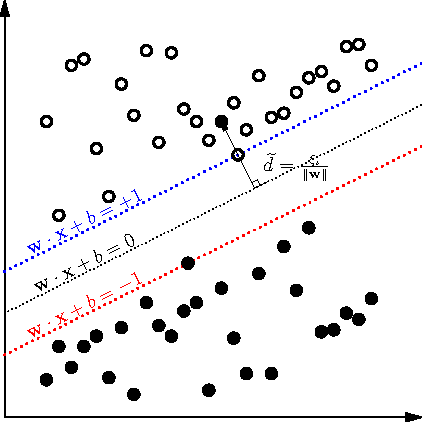
\includegraphics[scale=0.8]{fig/d2.pdf}
  \label{fig:d2}
\end{figure}

\noindent Introduce \emph{positive slack variables} $\ds\{\xi_i\}_{i=1}^m$ into the constraints
\begingroup
\addtolength{\jot}{-3pt}
\begin{align*}
  \vw\cdot\vx_i + b \geqslant +1 - \xi_i &\qquad\text{for }\,y_i=+1\\
  \vw\cdot\vx_i + b \leqslant -1 + \xi_i &\qquad\text{for }\,y_i=-1\\
  \xi_i\geqslant 0  &\qquad i=1,\,2,\,\ldots,\,m.
\end{align*}
\endgroup
The first two can be combined into
\begin{align*}
  1 - \xi_i - y_i\left(\vw\cdot\vx_i + b \right)\leqslant 0,\qquad i=1,\,2,\,\ldots,\,m
\end{align*}
If error occurs, $\xi_i > 1$; the objective function is changed to
\begin{align*}
  \text{minimize}\quad\frac{1}{2}\,\|\vw\|^2 + c\sum_{i=1}^m \xi_i
\end{align*}
where $c > 0$ controls the tolerance to errors on the training set. \\The Lagrangian with $2m$ multipliers $\lambda_i\geqslant 0$ and KKT conditions are
\begin{align}\label{f:lag1}
  \mathcal{L} = \frac{1}{2}\,\|\vw\|^2 + c\sum_{i=1}^m\xi_i + \sum_{i=1}^m\lambda_i\left\{1 - \xi_i - y_i\left(\vw\cdot\vx_i + b\right)\right\} - \sum_{i=1}^m\lambda_{m + i}\,\xi_i
\end{align}
\vspace{-8mm}
\begingroup
\addtolength{\jot}{-2pt}
\begin{equation}
\begin{aligned}\label{f:kkt1}
  &\frac{\partial\mathcal{L}}{\partial \vw} = 0 \ie \vw=\sum_{i=1}^m\lambda_i\,y_i\,\vx_i &\\
  &\frac{\partial\mathcal{L}}{\partial b} = 0 \ie \sum_{i=1}^m\lambda_iy_i=0 & \\
  &\frac{\partial\mathcal{L}}{\partial\xi_i} = 0 \ie c - \lambda_i-\lambda_{m + i} = 0, &i=1,\,2,\,\ldots,\,m\\
&\lambda_i\left\{1 - \xi_i - y_i\left(\vw\cdot\vx_i + b \right)\right\} = 0, &i=1,\,2,\,\ldots,\,m \\
  &1 - \xi_i - y_i\left(\vw\cdot\vx_i + b \right)\leqslant 0,\; &i=1,\,2,\,\ldots,\,m\\
  &\lambda_{m + i}\,\xi_i = 0,\quad\xi_i\geqslant 0, \quad & i=1,\,2,\,\ldots,\,m\\
  &\lambda_i\geqslant 0\qquad &i=1,\,2,\,\ldots,\,2m
\end{aligned}
\end{equation}
\endgroup
Substitute the KKT conditions (\ref{f:kkt1}) into $\mathcal{L}$ (\ref{f:lag1}), the dual Lagrangian 
\vspace{-1mm}
\begin{align*}
  \mathcal{L}_D=\sum_{i=1}^m\lambda_i-\frac{1}{2}\sum_{i=1}^m\sum_{j=1}^m\lambda_i\,\lambda_j\,y_i\,y_j\,\vx_i^\top\vx_j
\end{align*}
Now the problem becomes maximizing $\mathcal{L}_D$ subject to
\vspace{-1mm}
\begin{align*}
  0\leqslant\lambda_i\leqslant c\quad\text{and}\quad\sum_{i=1}^m\lambda_i y_i = 0.
\end{align*}

\newpage

\bibliographystyle{elsarticle-harv}
\bibliography{note11}

\end{document}
